
\documentclass[10pt,a4paper]{article}
\usepackage[utf8]{inputenc}
\usepackage[french]{babel}
\usepackage[left=2cm,right=2cm,top=2cm,bottom=2cm]{geometry}
\usepackage{hyperref}
\usepackage{graphicx}
\usepackage{amsmath,amssymb}
%opening
\title{TP}
\author{Nicolas Vadkerti}
\usepackage{listings} % Required for inserting code snippets
\usepackage[usenames,dvipsnames]{color} % Required for specifying custom colors and referring to colors by name

\definecolor{DarkGreen}{rgb}{0.0,0.4,0.0} % Comment color
\definecolor{highlight}{RGB}{255,251,204} % Code highlight color

\lstdefinestyle{Style1}{ % Define a style for your code snippet, multiple definitions can be made if, for example, you wish to insert multiple code snippets using different programming languages into one document
language=Perl, % Detects keywords, comments, strings, functions, etc for the language specified
backgroundcolor=\color{highlight}, % Set the background color for the snippet - useful for highlighting
basicstyle=\footnotesize\ttfamily, % The default font size and style of the code
breakatwhitespace=false, % If true, only allows line breaks at white space
breaklines=true, % Automatic line breaking (prevents code from protruding outside the box)
captionpos=b, % Sets the caption position: b for bottom; t for top
commentstyle=\usefont{T1}{pcr}{m}{sl}\color{DarkGreen}, % Style of comments within the code - dark green courier font
deletekeywords={}, % If you want to delete any keywords from the current language separate them by commas
%escapeinside={\%}, % This allows you to escape to LaTeX using the character in the bracket
firstnumber=1, % Line numbers begin at line 1
frame=single, % Frame around the code box, value can be: none, leftline, topline, bottomline, lines, single, shadowbox
frameround=tttt, % Rounds the corners of the frame for the top left, top right, bottom left and bottom right positions
keywordstyle=\color{Blue}\bf, % Functions are bold and blue
morekeywords={}, % Add any functions no included by default here separated by commas
numbers=left, % Location of line numbers, can take the values of: none, left, right
numbersep=10pt, % Distance of line numbers from the code box
numberstyle=\tiny\color{Gray}, % Style used for line numbers
rulecolor=\color{black}, % Frame border color
showstringspaces=false, % Don't put marks in string spaces
showtabs=false, % Display tabs in the code as lines
stepnumber=5, % The step distance between line numbers, i.e. how often will lines be numbered
stringstyle=\color{Purple}, % Strings are purple
tabsize=2
}

\newcommand{\insertcode}[2]{\begin{itemize}\item[]\lstinputlisting[caption=#2,label=#1,style=Style1]{#1}\end{itemize}} 


% \insertcode{"Scripts/example.pl"}{Nena would be proud.} 

\begin{document}

\maketitle

\section{HardWare}
Pour commencer, voici le montage qui nous permettra d'utiliser le moteur fourni celon les caractèristiques suivante : \\
Tension d'alimentaton du moteur : 24 Volts\\
Courant consommé par le moteur : 500 mA\\
\begin{figure}[h!]
\centering
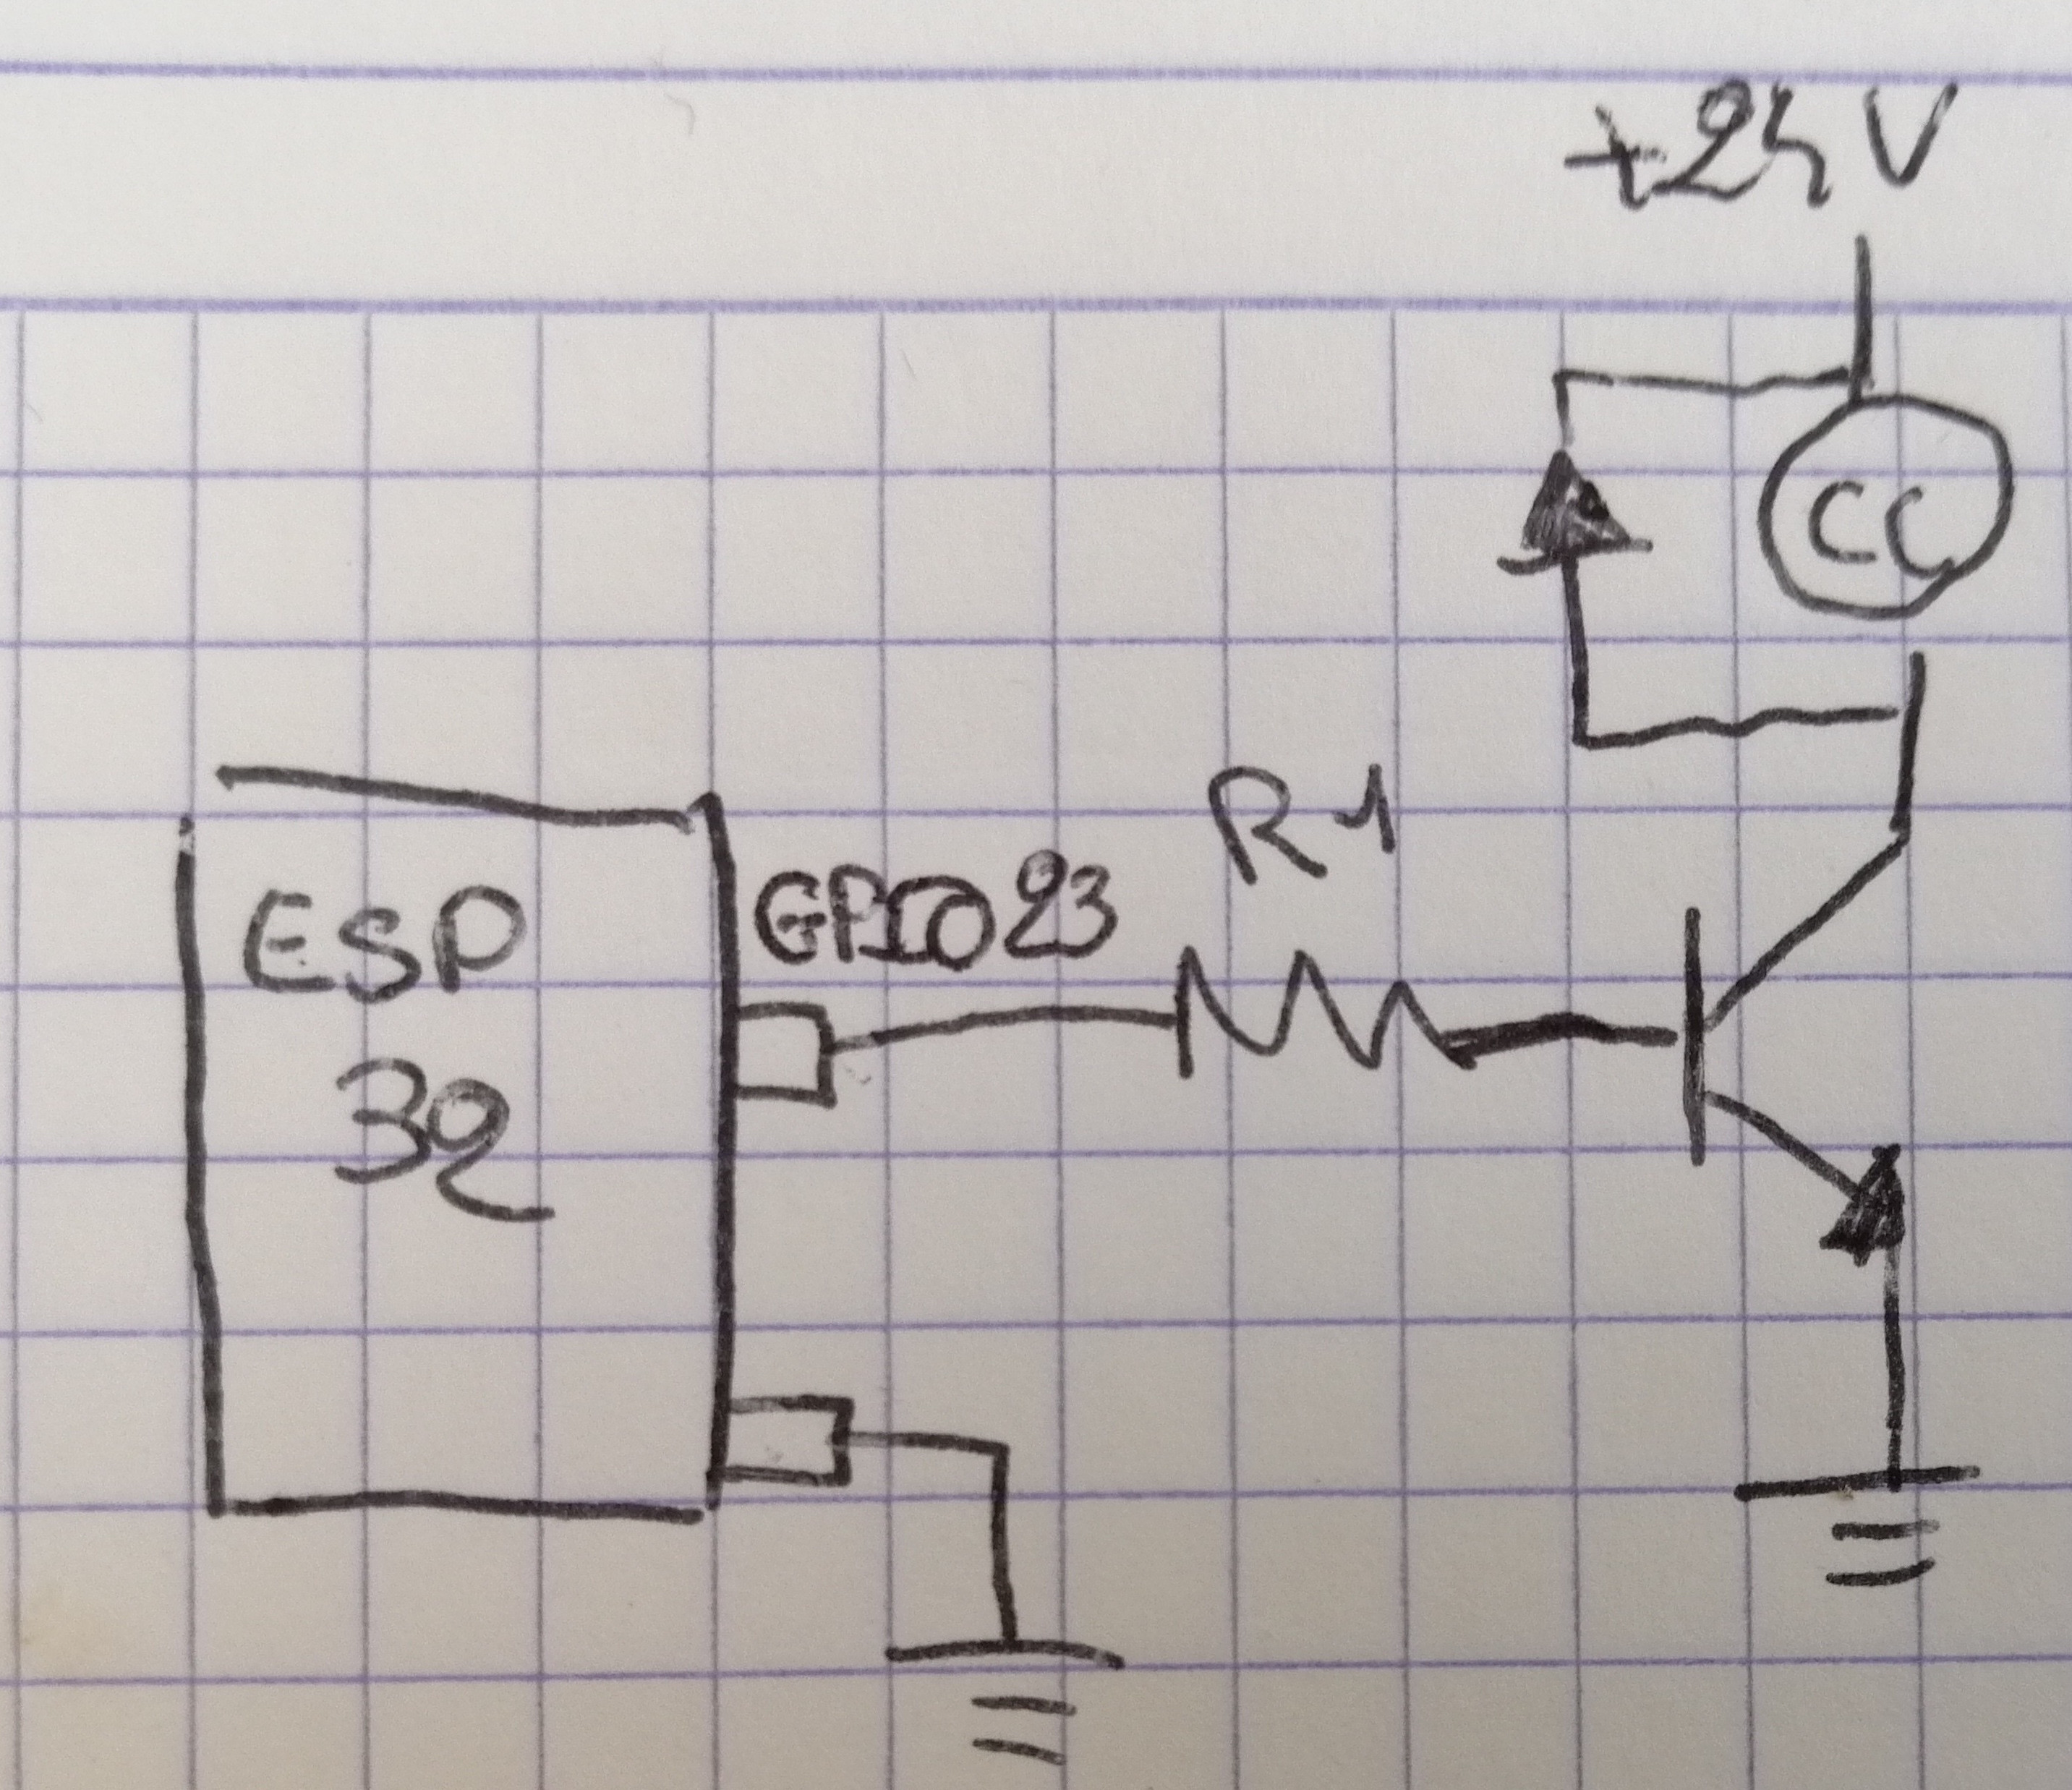
\includegraphics[scale=0.20]{image/1.jpg}
\caption{Montage }
\label{fig:net }
\end{figure}\\
Il faut donc calculer R1.\\
On suppose que le $\beta$ de notre transistor est de $\beta =100$ donc si on veut 500mA pour notre moteur, il faut appliquer à la base 0,005 A car 
$i_b=\frac{i_c}{\beta}=\frac{500mA}{100}=5mA $\\
Donc $R_1 = \frac{3,3V -0,7V(valeurTypique pour un transistor)}{0,005}=520\Omega$


Pour la diode de roue libre, il suffit quelle soit capable de laisser traverser 500mA et 24V 
 Ainsi nous pouront utilser notre moteur en utilisant un signal PWM via notre pin GPIO. En effetle transistor sera passant quand le GPIO sera à l'etat Haut, et le transistor sera bloquant quand le gpio sera a l'etat bas. Ainsi le signal pwm sera bien appliquer au moteur
 
 
 
 
\section{Communiquer avec l'objet communiquant}


L'idée est simple, l'ESP32 devra faire office de point d'accées Wifi. Il devra donc remplir les service de base pour etre facile d'utilisation pour le client. En effet, il devra, au moins faire serveur DHCP et serveur HTTP, pour que le client communique facilement avec celui à l'aide d'une page Web. Ainsi mis en place, L'esp32 mettra à jour regulierement les informations sur la page web qu'il ``pushera'' au client et lira les requetes ``POST'' du clients, et modifira donc la rotations du moteurs en conséquence. 
 
 \section{Le SoftWare pour l'ESP32}
 
On crée un serveur HTTP sur l'ESP32, on fait deux boutons, qui renvoie vers des urls distincts et quand l'utilisateur fais une requete sur cette url, la vitesse du moteurs change voici comment procéder :\newpage
\insertcode{code/code.ino}{Mon Code}
Le code compile, mais vu les conditions due au COVID-19, je ne peux pas tester si cela est fonctionnel. 



\end{document}

